\section{Background Theory}

\subsection{Overview}
This section is designed to present related background theory to assist in the
understanding of how the web interface works. The reader will become
familiarised with the key technologies behind the web interface, to allow a
greater understanding of how the components interacts with Tiberius and the
user.

%should you not \ref{tibby} rather than cite it!
Some of these concepts have been previously described in our preliminary report \cite{tibby-lit-review}, so technologies described in this section are kept sucinct. Elaboration of unfamiliar technologies can be found in the glossary.

% An overview of
% the technologies discussed is given below:

% \begin{description}[align=left]
% \item [MVC] is a the Model-View-Controller design pattern, and is most commonly
% used in web frameworks such as Django.

% \item [Django] is a popular web framework, used for small scale application
% such as this one, to large commercial applications.

% \end{description}
% Further definitions


\subsection{Django}
Django is a \gls{MVC} web framework, written in Python. The framework is designed for rapid development, suiting the requirements of this project well. Figure \ref{django-mvc} gives an overview of how the MVC architecture works.

% Diagram illustrating the internal structure of the Django framework.
\begin{figure}[!htb]
\begin{center}
\includegraphics[width=8cm]{api_mvc.png}
\end{center}
\caption{Django's MVC Architecture}
\label{fig:django-mvc}
\end{figure}

\begin{itemize}
\item A request is sent from the user's browser to the web server.
\item Django's URL Dispatcher matches the request URL with a View.
\item The View gets all data required to load the web page, from the Models.
\item The Models get their data from a data repository, a database in this case.
\item The View passes all it's data through the appropriate template, to get the HTML.
\item The HTML is returned to the browser by the view.
\end{itemize}

\subsection{Falcon}

Falcon is an open-source web framework for developing \glspl{API}. Falcon was particularly suited for our application because it is developed in Python, and it is extremely lightweight - meaning that it has hardly any dependencies.

The following will describe an example interaction between our \gls{webinterface} and our \gls{controlapi}, illustrating the chain of events that take place in the \gls{controlapi}.

Figure \ref{fig:api-falcon-simple} is a simplified representation of Falcon's core components. 

\begin{description}
\item{WSGI Servers} are web servers that implement the PEP 3333 Web Server Gateway Interface standard. These servers allow Python applications to run on them, by defining a universal interface between web servers and web applications \cite{pep-3333}.

\item [Application] Each Falcon application must create an instance of API. 

\item [Resource] The resource class is designed to be responsible for a particular type of resource. A diagrammatic representation of the resources we created can be found in Figure \ref{fig:api-modules}. Each resource class manages all requests delivered to the resource. Once the request has been dealt with, a HTTP response is returned to the source of the original request.

\item [Middleware] components define global behaviour that can occur before a request is passed on the the resource, or after the response has been created, but not yet sent. We have one middleware components that authenticates each incoming request before it is passed to a resource.
\end{description}

% Diagram illustrating simplified Falcon structure
\begin{figure}[!htb]
\begin{center}
\includegraphics[width=10cm]{api_falcon_simple.png}
\end{center}
\caption{Falcon Core Components}
\label{fig:api-falcon-simple}
\end{figure}



% Diagram illustrating the structure of the Falcon Framework
% \begin{figure}[!htb]
% \begin{center}
% 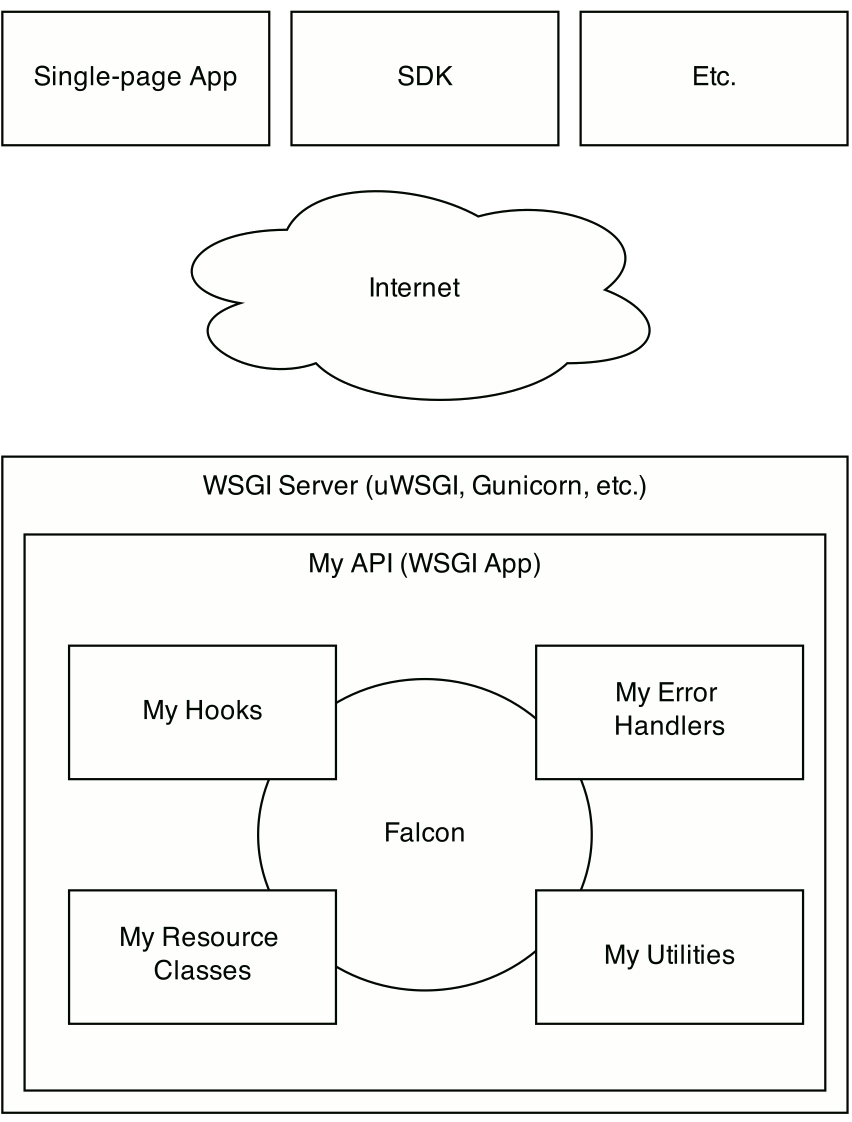
\includegraphics[width=12cm]{api_falcon.png}
% \end{center}
% \caption{Falcon Overview \cite{falcon-big-picture}}
% \label{fig:api-falcon}
% \end{figure}

